
\section{Tesztelés}

\subsection{Tesztelési terv}
\label{sec:tesztelesi_terv}

A rendszer tervezésének fontos részét képezi a funkcionális tesztelés. Leegyszerűsíti a megvalósítást, illetve segít elkerülni olyan hibákat, melyekre az imp\-le\-men\-tá\-lás során talán nem derülne fény. A rendszer étékelésének alapjául szolgál.

Teszteket érdemes modulonként végezni, ami után - feltételezve, hogy az egyes mo\-du\-lok működése megfelelő - a teljes rendszer tesztelése következhet. %Ehhez meg kell határozni, hogy melyik bemeneti adatra mi az elvárt viselkedés. Unit tesztek.
Az egyes modulok és feladatainak részletes leírása \aref{sec:interfesz_terv}.~fejezetben található. Az alábbiakban ezen modulok tesztelésének rövid leírása, majd a globális tesztelés következik.

\subsubsection{Modulok tesztelése}

A kliens és szerver közötti hálózaton történő kommunikációt megvalósító üzenetek előállításának, illetve a beérkező üzenetek elemzésének tesztelése szintén elengedhetetlen a helyes működéshez.

\subsubsection{Globális tesztelés}

\begin{figure}[htb]
\center
\resizebox{14.5cm}{!}{
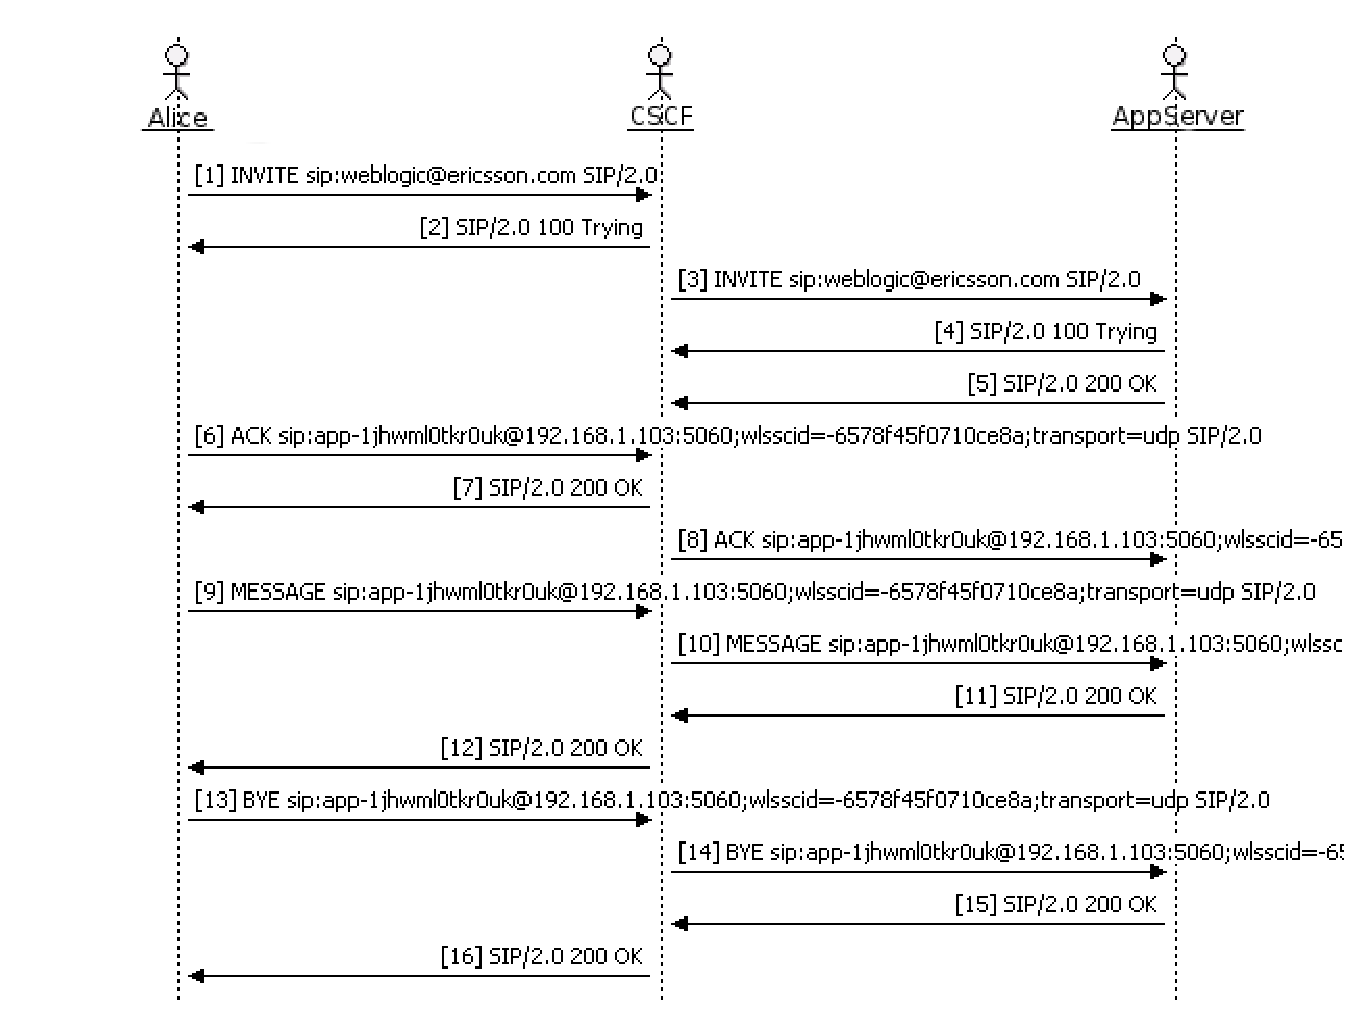
\includegraphics{img/vtf-kuldes-01.eps}}
\caption{Alice üzenetet küld a csoportnak}
\label{fig:teszt-vtf-kuldes-01}
\end{figure}

\begin{figure}[htb]
\center
\resizebox{14.5cm}{!}{
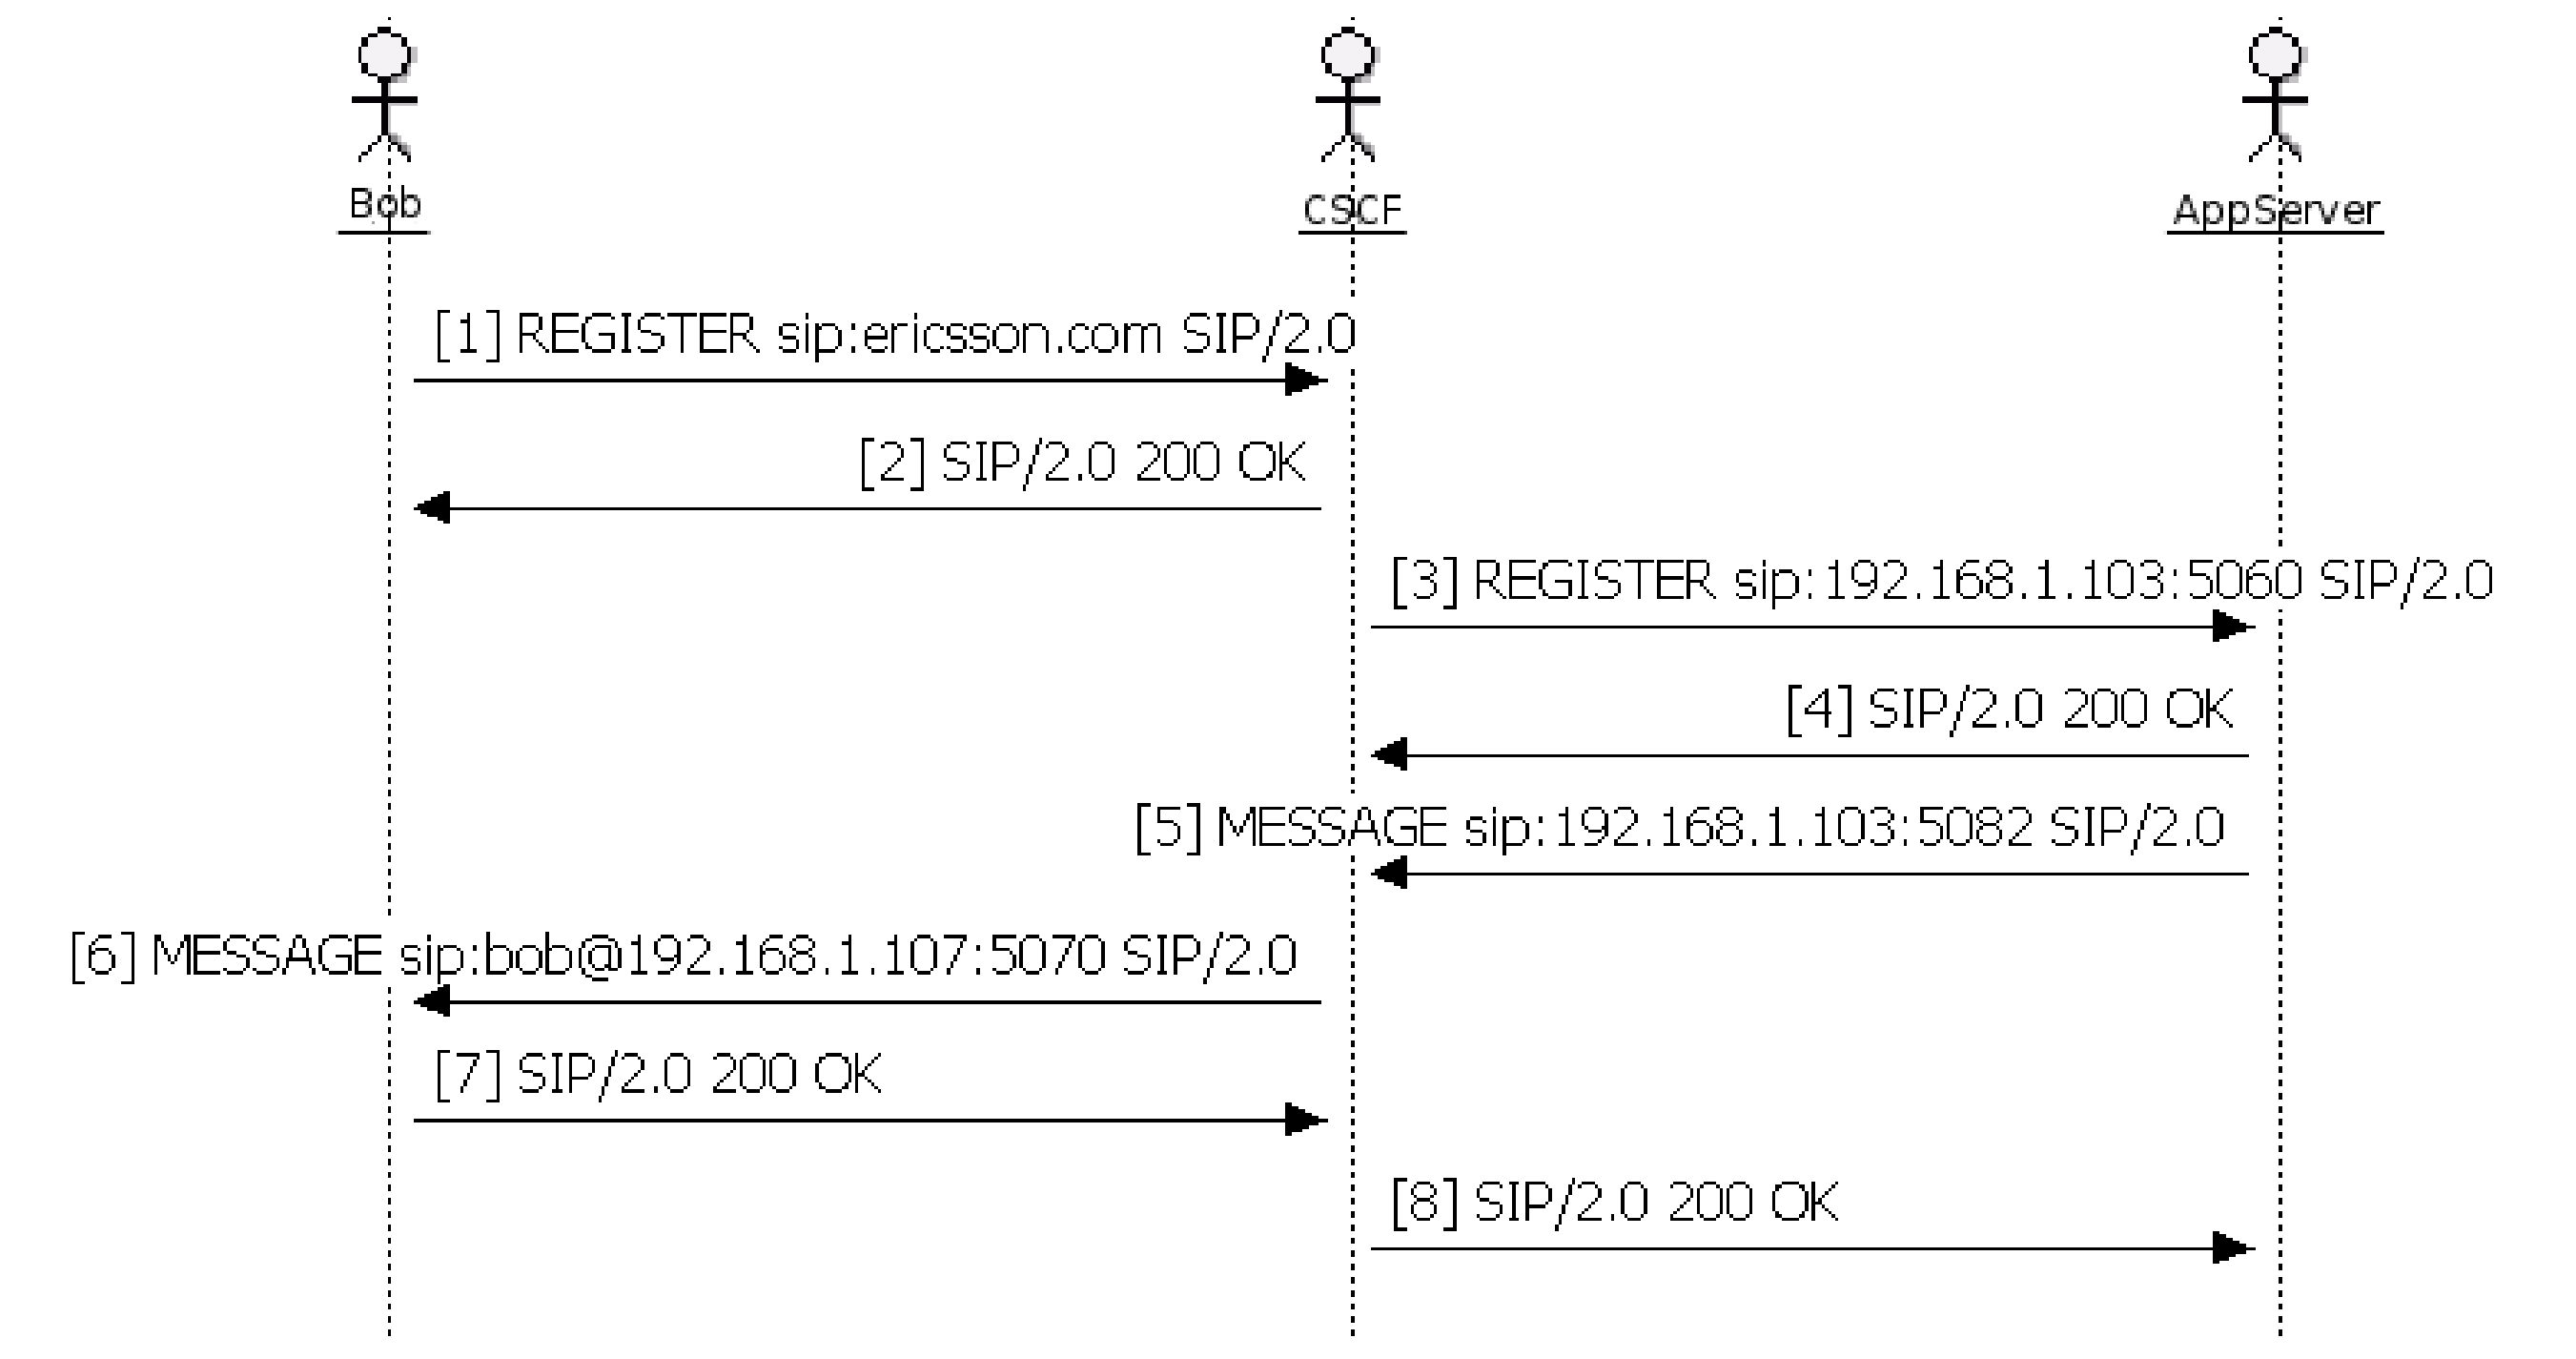
\includegraphics{img/vtf-kuldes-02.eps}}
\caption{A szolgáltatás értesíti Bob-ot az új üzeneteiről}
\label{fig:teszt-vtf-kuldes-01}
\end{figure}